
\documentclass{article}
\usepackage{amsmath}
\usepackage{xcolor}
\usepackage{ragged2e}
\usepackage{graphicx}
\begin{document}
\begin{center}
\color{cyan} EXERCISE 9.2
\end{center}
Write True or False and justify your answer:
\begin{enumerate}
	\item $ABCD$ is a parallelogram and $X$ s the mid-point of $AB$. If ar($AXCD$) = 24 \(cm^2\), then ar ($ABC$) = 24 \(cm^2\).
	\item $PQRS$ is a rectangle inscribed in a quadrant of a circle of radius 13 cm. $A$ is any point on $PQ$. If $PS$ = 5 cm, then ar ($PAS$) = 30 \(cm^2\).
	\item $PQRS$ is a parallelogram whose area is 180 \(cm^2\) and $A$ is any point on the diagonal $QS$. The area of $\triangle{ASR}$ = 90 \(cm^2\).
	\item $ABC$ and $BDE$ are two equilateral triangles such that $D$ is the mid-point of $BC$. Then
	\begin{align}
		{ar (BDE)} &= \frac{1}{4} {ar (ABC)}.
		\label{eq:9.24}
	\end{align}
\item    In Fig. \ref{fig:925}, $ABCD$ and $EFGD$ are     two parallelograms and $G$ is the mid-point of $CD$.Then
		\begin{align}
			{ar (DPC)} = \frac{1}{2} {ar (EFGD)}.
			\label{eq:9.25}
		\end{align}
\begin{figure}[h]
	\centering
	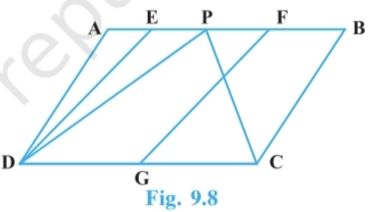
\includegraphics[width=\columnwidth]{figs/925.jpg}
	\caption{}
	\label{fig:925}
\end{figure}
\end{enumerate}
\end{document}
